% !TEX program = xelatex
\documentclass[UTF8,fontset=fandol,a4paper,11pt]{ctexart}
\usepackage[margin=21mm,top=23mm,bottom=22mm,headheight=16pt]{geometry}
\usepackage{amsmath,amssymb,mathtools,bm}
\usepackage{tikz}
\usetikzlibrary{arrows.meta,calc,angles,quotes,patterns}
\usepackage{xcolor,booktabs,array,longtable,enumitem,fancyhdr,needspace}
\usepackage[unicode,hidelinks]{hyperref}
\definecolor{ink}{HTML}{24343C}
\definecolor{accent}{HTML}{166A70}
\definecolor{muted}{HTML}{65747A}
\definecolor{rulegray}{HTML}{D4DDE0}
\definecolor{warm}{HTML}{966037}
\color{ink}
\setlength{\parindent}{2em}
\setlength{\parskip}{4pt}
\linespread{1.12}
\AtBeginDocument{\setlength{\abovedisplayskip}{6pt plus 2pt minus 1pt}
\setlength{\belowdisplayskip}{6pt plus 2pt minus 1pt}
\setlength{\abovedisplayshortskip}{0pt plus 1pt}
\setlength{\belowdisplayshortskip}{4pt plus 1pt}}
\setlist[enumerate]{label=(\arabic*),leftmargin=2.3em,itemsep=3pt,topsep=4pt}
\setlist[itemize]{leftmargin=2em,itemsep=2pt,topsep=4pt}
\allowdisplaybreaks[1]
\setlength{\emergencystretch}{2em}
\setcounter{secnumdepth}{0}
\providecommand{\tightlist}{\setlength{\itemsep}{0pt}\setlength{\parskip}{0pt}}
\ctexset{section={format=\Large\bfseries\color{accent},beforeskip=10pt,afterskip=9pt},
subsection={format=\normalsize\bfseries\color{accent},beforeskip=10pt,afterskip=4pt},
subsubsection={format=\normalsize\bfseries,beforeskip=8pt,afterskip=3pt}}
\pagestyle{fancy}
\fancyhf{}
\fancyhead[L]{\small\color{muted}物理学难题集萃}
% 页眉仅保留书名；版本名称只在封面显示。
\fancyfoot[L]{\small\color{muted}\chapterlabel}
\fancyfoot[R]{\small\thepage}
\renewcommand{\headrulewidth}{0.4pt}
\renewcommand{\footrulewidth}{0pt}
\newcommand{\dd}{\mathop{}\!\mathrm{d}}
\newcommand{\vect}[1]{\bm{#1}}
\newcommand{\tagline}[1]{\noindent{\small\color{muted}#1}\par}
\newcommand{\result}[1]{\begin{equation*}\boxed{#1}\end{equation*}}
\newcommand{\figcaption}[1]{\par\vspace{2pt}{\small\color{muted}#1}\par}
\newcommand{\teach}[2]{\Needspace{4\baselineskip}\subsection*{讲解要点与追问}#1\par\smallskip\noindent\textbf{追问：}#2\par}
\newcommand{\workarea}{\par\vspace{7mm}\noindent{\small\color{muted}作答区}\par\vspace{4mm}
\noindent\textcolor{rulegray}{\rule{\linewidth}{0.3pt}}\par\vspace{16mm}
\noindent\textcolor{rulegray}{\rule{\linewidth}{0.3pt}}\par\vspace{16mm}
\noindent\textcolor{rulegray}{\rule{\linewidth}{0.3pt}}\par\vspace{16mm}
\noindent\textcolor{rulegray}{\rule{\linewidth}{0.3pt}}}
\tikzset{axis/.style={-{Stealth[length=2mm]},thin,color=muted},
motion/.style={-{Stealth[length=2.3mm]},thick,color=accent},
force/.style={-{Stealth[length=2.3mm]},thick,color=warm},
traj/.style={thick,color=accent},guide/.style={dashed,thin,color=muted},
object/.style={thick,color=ink},every node/.style={font=\small}}\widowpenalty=10000\clubpenalty=10000\displaywidowpenalty=10000\newcommand{\chapterlabel}{综合试题（一）}







\hypersetup{pdftitle={综合试题（一）·学生版},pdfauthor={}}

\begin{document}\pdfbookmark[0]{综合试题（一）}{cover}

\thispagestyle{empty}\vspace*{22mm}

\noindent{\Huge\bfseries 物理学难题集萃}\par\vspace{12mm}

\noindent{\LARGE 综合试题（一）}\par\vspace{12mm}

\noindent{\Large\color{accent}学生版}\par\vspace{9mm}

\noindent\textcolor{accent}{\rule{\linewidth}{1pt}}\par\vspace{9mm}

\noindent 第1--6题\par\vfill\clearpage

\pdfbookmark[1]{题目目录}{contents}\section*{题目目录}

\begin{longtable}{@{}r p{113mm} r@{}}\toprule 题号 & 题目 & 页码\\\midrule

\hyperref[q:1]{1} & \hyperref[q:1]{内盘与外环的两阶段摩擦运动} & \pageref{q:1} \\

\hyperref[q:2]{2} & \hyperref[q:2]{椭圆轨道的引力规律与彗星速度} & \pageref{q:2} \\

\hyperref[q:3]{3} & \hyperref[q:3]{四维理想气体的统计规律和热过程} & \pageref{q:3} \\

\hyperref[q:4]{4} & \hyperref[q:4]{三个频率电源的稳态电流与平均功率} & \pageref{q:4} \\

\hyperref[q:5]{5} & \hyperref[q:5]{幂律径向电场中的粒子束聚焦} & \pageref{q:5} \\

\hyperref[q:6]{6} & \hyperref[q:6]{列车入隧道与机械扰动的传播} & \pageref{q:6} \\

\bottomrule\end{longtable}

\clearpage

\pdfbookmark[2]{第 1 题 内盘与外环的两阶段摩擦运动}{q1}

\section*{第 1 题\quad 内盘与外环的两阶段摩擦运动}\label{q:1}


从半径$2R$的均匀薄圆盘中央切出半径$R$的圆盘，切缝很窄，得到质量$m$的内盘和质量$3m$的外环。二者竖立于水平地面，初始共同向右平动，速度$v_0$，均不转动。外环与地面间滑动摩擦因数$\mu_0=0.5$，内盘与外环间滑动摩擦因数为$\mu$，静摩擦的最大比值也取$\mu$；地面静摩擦上限取$0.5$倍法向力。重力加速度$g$。

忽略窄缝造成的两圆心位移及接触点迁移的短暂过程，视为两圆心有相同水平加速度，竖直位置不变。
\begin{enumerate}
\item 求内盘与外环间出现相对滑动的$\mu$范围。
\item 取$\mu=0.2$，讨论地面由滑动变为无滑滚动前后的运动，求最终共同平动速度。列出两阶段加速度及转换条件，并检查地面静摩擦是否足够。
\end{enumerate}


\begin{center}\begin{minipage}{.98\linewidth}\centering
\begin{tikzpicture}[scale=.8,transform shape]

\draw[object] (0,0) circle (2); \draw[object] (0,0) circle (1.03);
\draw[object] (0,0) circle (.98);
\draw[object] (-3,-2)--(3.8,-2);
\fill (0,0) circle (1.5pt) node[above left] {$O$};
\draw[guide] (0,0)--(45:2) node[pos=.82,above left] {$2R$};
\draw[guide] (0,0)--(-35:1) node[midway,above] {$R$};
\node at (-.4,.5) {$m$};\node at (-1.45,.5) {$3m$};
\draw[motion] (2.4,.6)--(4.3,.6) node[right] {$v_0$};
\node[below] at (0,-2.2) {地面：$\mu_0=0.5$};
\node[align=left] at (6.3,-.3) {内接触：$\mu$\\初始两者均不转\\切缝与中心位移略去};

\end{tikzpicture}
\figcaption{图综一.1\quad 外环外半径2R，内盘半径R；最初共同平动。}
\end{minipage}\end{center}

\par\vspace{5mm}\noindent{\small\color{muted}作答区}\par\vspace{3mm}\noindent\textcolor{rulegray}{\rule{\linewidth}{0.3pt}}\par\vspace{12mm}\noindent\textcolor{rulegray}{\rule{\linewidth}{0.3pt}}

\clearpage

\pdfbookmark[2]{第 2 题 椭圆轨道的引力规律与彗星速度}{q2}

\section*{第 2 题\quad 椭圆轨道的引力规律与彗星速度}\label{q:2}


一小天体在指向固定太阳的中心力作用下沿非圆椭圆运动，椭圆长、短半轴分别为$A>B>0$，力的大小为$F=GMm/r^\alpha$，比例系数的量纲随$\alpha$取值相应确定。
\begin{enumerate}
\item 若太阳位于（a）椭圆中心，（b）椭圆一个焦点，分别求$\alpha$。除必要条件外，还应说明对应的力确可产生整条椭圆。
\item 在平方反比引力下：（a）求近日点速度及轨道周期；（b）利用图中的彗星绕木星轨道和时间标记，估算近木点速度。图为测量示意，长轴与短轴的纸面长度约为$5.6\,\mathrm{cm}$和$0.30\,\mathrm{cm}$，比例尺$3.5\,\mathrm{cm}$对应$3.0\times10^7\,\mathrm{km}$；1993年7月1日约在远木点，1994年7月16日接近近木端。可把这一时间间隔粗取$380\,\mathrm d$。
\end{enumerate}
讨论把形式近木点速度直接当作进入大气层速度的条件。另取大气入口距木星中心$r_{\rm atm}=7.1\times10^4\,\mathrm{km}$，按同一轨道模型估算该处速度。忽略太阳扰动及大气阻力；一天取$86400\,\mathrm s$。


\begin{center}\begin{minipage}{.98\linewidth}\centering
\begin{tikzpicture}[scale=.8,transform shape]

\draw[object] (0,0) ellipse (2 and 1);
\fill (0,0) circle (2pt) node[below] {中心力心};
\draw[axis] (-2.4,0)--(2.4,0);
\draw[axis] (0,-1.4)--(0,1.4);
\node at (0,2) {（a）};
\begin{scope}[xshift=6cm]
\draw[object] (0,0) ellipse (2 and 1);
\fill (-1.732,0) circle (2pt) node[below] {焦点力心};
\draw[axis] (-2.4,0)--(2.4,0);
\node at (0,2) {（b）};
\end{scope}
\begin{scope}[yshift=-4cm,xshift=3cm,rotate=-20]
\draw[object] (0,0) ellipse (2.8 and .15);
\fill (-2.795979,0) circle (2pt);
\node[above left,rotate=0] at (-2.8,0) {木星、近木端：1994.7.16};
\node[below right,rotate=0] at (2.8,0) {远木端：1993.7.1};
\end{scope}
\draw[axis,<->] (0,-6)--(3.5,-6);
\foreach \x/\s in {0/0,1.1667/10,2.3333/20,3.5/30}{\draw (\x,-5.85)--(\x,-6.15) node[below] {$\s$};}
\node[right] at (4,-6) {$10^6\,\mathrm{km}$};

\end{tikzpicture}
\figcaption{图综一.2\quad 两种力心位置与彗星的极扁轨道测量示意。}
\end{minipage}\end{center}

\par\vspace{5mm}\noindent{\small\color{muted}作答区}\par\vspace{3mm}\noindent\textcolor{rulegray}{\rule{\linewidth}{0.3pt}}\par\vspace{12mm}\noindent\textcolor{rulegray}{\rule{\linewidth}{0.3pt}}

\clearpage

\pdfbookmark[2]{第 3 题 四维理想气体的统计规律和热过程}{q3}

\section*{第 3 题\quad 四维理想气体的统计规律和热过程}\label{q:3}


设想四维欧氏空间中的单原子理想气体，分子质量为$m$，温度为$T$，四个直角坐标方向等价且相互独立。气体占有的四维体积记为$V_4$，分子数$N$，物质的量$\nu=N/N_A$，$R=N_Ak_B$。
\begin{enumerate}
\item 分别求：（a）方均根速率；（b）四维速度矢量的归一化概率密度$F_4(v_1,v_2,v_3,v_4)$；（c）速率概率密度$f_4(v)$；（d）平均速率。推导四维速度壳的几何因子。
\item 四维压强定义为单位三维超面积上的法向力，气体做功仍记作$p\,dV_4$。求：（a）状态方程；（b）绝热过程$p$与$V_4$关系；（c）在$p$正比于$V_4$的直线过程中，摩尔热容$C$。结果用$R$表示，并写出一般常热容多方过程关系。
\end{enumerate}


\begin{center}\begin{minipage}{.98\linewidth}\centering
\begin{tikzpicture}[scale=.8,transform shape]

\draw[axis] (0,0)--(3.4,0) node[right] {$v_1$};
\draw[axis] (0,0)--(0,2.5) node[above] {$v_2$};
\draw[axis] (0,0)--(-1.8,-1.4) node[below left] {$v_3$};
\draw[axis] (0,0)--(1.8,-1.5) node[below right] {$v_4$};
\node[align=left] at (6,1.5) {四个独立分量\\$v^2=\sum_{i=1}^4v_i^2$};
\begin{scope}[xshift=5cm,yshift=-2cm]
\draw[axis] (0,0)--(4,0) node[right] {$V_4$};
\draw[axis] (0,0)--(0,2.5) node[above] {$p$};
\draw[traj] (0,0)--(3.5,2.1) node[right] {$p=aV_4$};
\end{scope}

\end{tikzpicture}
\figcaption{图综一.3\quad 四个速度坐标的符号投影及所求热过程路径。}
\end{minipage}\end{center}

\par\vspace{5mm}\noindent{\small\color{muted}作答区}\par\vspace{3mm}\noindent\textcolor{rulegray}{\rule{\linewidth}{0.3pt}}\par\vspace{12mm}\noindent\textcolor{rulegray}{\rule{\linewidth}{0.3pt}}

\clearpage

\pdfbookmark[2]{第 4 题 三个频率电源的稳态电流与平均功率}{q4}

\section*{第 4 题\quad 三个频率电源的稳态电流与平均功率}\label{q:4}


理想电压源、电阻、电感和电容按图连接。底部导线为参考电势零；左电源$\mathcal E_1$使左侧电阻端电势升为$\mathcal E_1$，中、右两电源$\mathcal E_2,\mathcal E_3$的电势升高方向均向下。电阻电流$i$正方向向上经过左支路，再由左向右流过电阻。
\[
\begin{aligned}
\mathcal E_1&=E_0\cos(\tfrac12\omega t+30^\circ),\\
\mathcal E_2&=E_0\cos(\omega t+45^\circ),\\
\mathcal E_3&=E_0\cos(2\omega t+60^\circ).
\end{aligned}
\]
已知$\omega L=1/(\omega C)=R$。求电阻的稳态电流$i(t)$，并求长时间平均消耗功率。须写出逐频率叠加和时间平均的依据。


\begin{center}\begin{minipage}{.98\linewidth}\centering
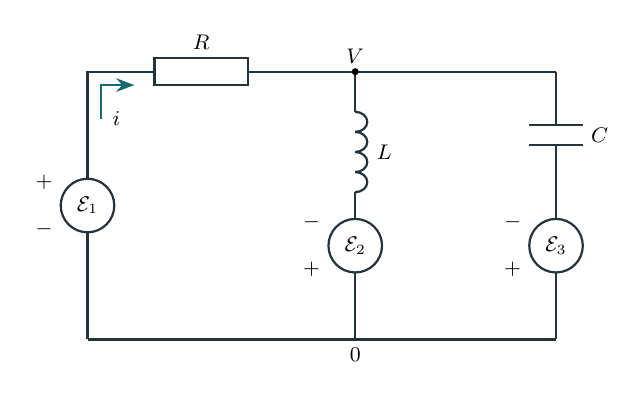
\begin{tikzpicture}[scale=.85,transform shape]

\draw[object] (0,0)--(0,1.6); \draw[object] (0,2.4)--(0,4)--(1,4);
\draw[object] (1,3.8) rectangle (2.4,4.2); \node[above] at (1.7,4.2) {$R$};
\draw[object] (2.4,4)--(7,4);
\draw[object] (0,0)--(7,0);
\draw[object] (0,2) circle (.4); \node at (0,2) {$\mathcal E_1$};
\node[left] at (-.4,2.35) {$+$};\node[left] at (-.4,1.65) {$-$};
\draw[object] (4,4)--(4,3.4);
\foreach \y in {3.4,3.1,2.8,2.5}{\draw[object] (4,\y) arc[start angle=90,end angle=-90,x radius=.18,y radius=.15];}
\node[right] at (4.2,2.8) {$L$};
\draw[object] (4,2.2)--(4,1.8); \draw[object] (4,1.4) circle (.4);
\draw[object] (4,1)--(4,0);
\node at (4,1.4) {$\mathcal E_2$};
\node[left] at (3.6,1.75) {$-$};\node[left] at (3.6,1.05) {$+$};
\draw[object] (7,4)--(7,3.2); \draw[object] (6.6,3.2)--(7.4,3.2);
\draw[object] (6.6,2.9)--(7.4,2.9); \draw[object] (7,2.9)--(7,1.8);
\node[right] at (7.4,3.05) {$C$};
\draw[object] (7,1.4) circle (.4); \node at (7,1.4) {$\mathcal E_3$};
\draw[object] (7,1)--(7,0);
\node[left] at (6.6,1.75) {$-$};\node[left] at (6.6,1.05) {$+$};
\draw[motion] (.2,3.3)--(.2,3.8)--(.7,3.8);
\node[right] at (.25,3.3) {$i$};
\fill (4,4) circle (1.5pt) node[above] {$V$};
\node[below] at (4,0) {$0$};

\end{tikzpicture}
\figcaption{图综一.4\quad 电源极性与电阻电流方向；三电源的频率依次为$\omega/2$、$\omega$、$2\omega$。}
\end{minipage}\end{center}

\par\vspace{5mm}\noindent{\small\color{muted}作答区}\par\vspace{3mm}\noindent\textcolor{rulegray}{\rule{\linewidth}{0.3pt}}\par\vspace{12mm}\noindent\textcolor{rulegray}{\rule{\linewidth}{0.3pt}}

\clearpage

\pdfbookmark[2]{第 5 题 幂律径向电场中的粒子束聚焦}{q5}

\section*{第 5 题\quad 幂律径向电场中的粒子束聚焦}\label{q:5}


平面内有径向电场$\boldsymbol E=-\kappa r^{-\beta}\hat{\boldsymbol r}$，其中$\kappa>0$、$\beta\ne1$。质量$m$、正电荷$q$的粒子从$S$发射，不计粒子间作用、重力和辐射。
\begin{enumerate}
\item 粒子以切向速度$v_0$沿半径$r_0$的圆轨道运动，求$r_0$。
\item 发射速率均为$v_0$，方向相对圆轨道切线有小角度偏离：最外射线偏外$\alpha_{\rm out}$，最内射线偏内$\alpha_{\rm in}$，总角宽$\alpha=\alpha_{\rm out}+\alpha_{\rm in}\ll1$。求使粒子在距中心$r_0$处重新聚焦的$\beta$范围、第一次聚焦的方位角$\phi_1$，以及方位角$\phi_1/2$处的径向束宽。取$\beta=-13$，画出粒子从$S$到转过$2\pi$的轨迹示意。
\item 在上述可聚焦范围内，改为方向均沿切线，速率分布在$v_0$至$v_0+\Delta v$，其中$\Delta v/v_0\ll1$。求第一次聚焦角$\phi_2$及方位角$\phi_2/2$处径向束宽；同样画$\beta=-13$时的轨迹。
\end{enumerate}
聚焦位置和束宽均求小角度、小相对速度差的一阶近似，说明稳定性和近似条件。


\begin{center}\begin{minipage}{.98\linewidth}\centering
\begin{tikzpicture}[scale=.8,transform shape]

\draw[object] (0,0) circle (2.5);
\fill (0,0) circle (2pt) node[below left] {$O$};
\fill (2.5,0) circle (2pt) node[below right] {$S$};
\draw[guide] (0,0)--(2.5,0) node[midway,below] {$r_0$};
\draw[motion] (2.5,0)--(2.5,2) node[above] {$v_0$切向};
\draw[motion] (2.5,0)--(3.1,1.9);
\draw[motion] (2.5,0)--(1.9,1.9);
\draw[force] (1.77,1.77)--(.85,.85) node[midway,above left] {$q\boldsymbol E$};
\draw[axis] (.8,0) arc[start angle=0,end angle=55,radius=.8];
\node at (.95,.5) {$\theta$};
\node[align=left] at (6,.4) {（2）小角宽$\alpha$\\（3）切向速度展宽$\Delta v$\\$\boldsymbol E=-\kappa r^{-\beta}\hat{\boldsymbol r}$};

\end{tikzpicture}
\figcaption{图综一.5\quad 参考圆、径向电力与两种发射展宽条件。}
\end{minipage}\end{center}

\par\vspace{5mm}\noindent{\small\color{muted}作答区}\par\vspace{3mm}\noindent\textcolor{rulegray}{\rule{\linewidth}{0.3pt}}\par\vspace{12mm}\noindent\textcolor{rulegray}{\rule{\linewidth}{0.3pt}}

\clearpage

\pdfbookmark[2]{第 6 题 列车入隧道与机械扰动的传播}{q6}

\section*{第 6 题\quad 列车入隧道与机械扰动的传播}\label{q:6}


隧道$A_1B_1$静止长度为$L_1$，列车$A_2B_2$自身静止长度为$L_2>L_1$。列车向左运动，$A_2$为前端，$B_2$为后端，隧道左端$A_1$是封闭挡墙，右端$B_1$设一扇门。
\begin{enumerate}
\item 选择速度$v$，使地面惯性系$S_1$中，前端$A_2$到达左墙$A_1$与后端$B_2$到达右门$B_1$两事件同时发生，求$v$。
\item 在列车碰撞前的静止惯性系$S_2$中，上述哪一事件先发生？两事件的时间间隔$\Delta t_2$是多少？即使列车后来发生碰撞，也继续使用这个惯性系。
\item 门在$S_1$所述同时事件处关上。用一个理想传播模型描述碰撞：前端一碰墙便随墙向右运动，而使车体运动状态改变的机械扰动从前端向后端传播；在尚未受扰的列车惯性系$S_2$中，传播速度为$u>0$，后端在扰动到达前保持静止。要使门到达并关住后端不晚于扰动到达后端，$u$应满足什么上界？
\end{enumerate}
若进一步假设这种材料的$u$不随$v$及所选$L_2$改变，并要求对任意满足第（1）问的列车与隧道均成立，证明$u\leq c$。这里讨论扰动到达的因果条件，不要求求解车体的具体压缩过程。


\begin{center}\begin{minipage}{.98\linewidth}\centering
\begin{tikzpicture}[scale=.8,transform shape]

\draw[object] (0,1)--(0,-.2)--(6,-.2)--(6,1);
\node[above] at (0,1) {$A_1$墙};\node[above] at (6,1) {$B_1$门};
\draw[axis,<->] (0,-1)--(6,-1) node[midway,below] {$L_1$};
\draw[object] (0,.1) rectangle (6,.65);
\node[below left] at (0,.1) {$A_2$};
\node[below right] at (6,.1) {$B_2$};
\draw[motion] (3,1.8)--(1,1.8) node[left] {$v$};
\node[right] at (7,.5) {$S_1$中恰好同时容纳};
\node at (3,-2.5) {列车碰撞前静长$L_2>L_1$，运动方向向左};

\end{tikzpicture}
\figcaption{图综一.6\quad 地面系中两个端点相遇事件同时发生，图示运动长度为L1。}
\end{minipage}\end{center}

\par\vspace{5mm}\noindent{\small\color{muted}作答区}\par\vspace{3mm}\noindent\textcolor{rulegray}{\rule{\linewidth}{0.3pt}}\par\vspace{12mm}\noindent\textcolor{rulegray}{\rule{\linewidth}{0.3pt}}

\end{document}
